% CVS info
\RCS$Revision: 1.5 $
\RCS$Date: 2008/09/06 05:57:25 $
%%%%%%%%%%%%% ptdr definitions %%%%%%%%%%%%%%%%%%%%%

%------------------------------------------------------------------------------
%%% put your own definitions here:
 
%%%%%%%%%%%%%%%%
% Declarations %
%%%%%%%%%%%%%%%%
%\def\bb{$\mathrm{b}\overline{\mathrm{b}}\;$}
%\def\cc{$\mathrm{c}\overline{\mathrm{c}}\;$}
\def\bb{$b\overline{b}\;$}
\def\cc{$c\overline{c}\;$}
\def\ttbar{$t\overline{t}\;$}
\def\mttbar{$m_{t\overline{t}}\;$}
\def\Zp{${Z'}\;$}
\def\ddZ{$\mathrm{d}\overline{\mathrm{d}}$}
\def\ss{$\mathrm{s}\overline{\mathrm{s}}\;$}
%\def\ttbar{$\mathrm{t}\overline{\mathrm{t}}\;$}
\def\ssZ{$\mathrm{s}\overline{\mathrm{s}}$}
\def\zqq{$\mathrm{Z} \rightarrow \mathrm{q}\overline{\mathrm{q}}\;$}
\def\zcc{$\mathrm{Z} \rightarrow \mathrm{c}\overline{\mathrm{c}}\;$}
\def\zbb{$\mathrm{Z} \rightarrow \mathrm{b}\overline{\mathrm{b}}\;$}
\def\zuuZ{$\mathrm{Z} \rightarrow \mathrm{u}\overline{\mathrm{u}}$}
%\def\gev{~GeV/$c\;$}
\def\gevc{~GeV/$c\;$}
\def\gevcc{~GeV/$c^{2}\;$}
\def\mum{~$\mu$m$\;$}
\def\pt{$p_T\;$}
\def\ptZ{$p_T$}
\def\Et{$E_T\;$}
\def\EtZ{$E_T$}
\def\ip{$IP\;$}
\def\ipZ{$IP$}
\def\dca{$dca\;$}
\def\prob{${\cal P}_{jet}\;$}
\def\probZ{${\cal P}_{jet}$}
\def\dr{$\Delta R\;$}
\def\pscat{$p_{scat}\;$}
\def\pscatZ{$p_{scat}$}
\def\sip{${\cal S}_{IP}\;$}
%\def\ptrel{$p_T^{\rm rel}}
\def\ptrel{$p_{Trel}\;$}
%\def\ptrelZ{$p_{Trel}$}
\def\tag{${\cal P}_{jet}^+<$}
%%%%%%%%%%%%%%%  Title page %%%%%%%%%%%%%%%%%%%%%%%%
% select one of the following and type in the proper number:
\cmsNoteHeader{2008/081}

\title{\bf Measurement of the $b$ tagging Performance using a Muon in Jets Sample: Update of the System8 Method with the CSA07 MC samples.}

%\author[fnal]{PRELIMINARY AUTHOR LIST}
\author[purdue]{P.~Jindal}
\author[fnal]{F.~Yumiceva}
\address[fnal]{Fermi National Accelerator Laboratory, Batavia, Illinois USA}  
\address[purdue]{Purdue University Calumet, Hammond, Indiana, USA}
\date{\today}
  
\abstract{
This note describes the improvements developed since the analysis note CMS AN 2007/046 using the CSA07 MC samples. The System8 method has been 
extended to consider correlations for the soft muon tagger. In this 
case the soft muon tagger is a simple tagger based only in the 
$p_{Trel}$ distribution. We also study the System8 convergency 
and developed options to choose the best solution in case multiple 
solutions are available. As a results, the convergency range 
in jet $p_T$ of this
method has been extended compared to the previous analysis.
}

% these need to be filled in by hand
\hypersetup{%
pdfauthor={Francisco Yumiceva},%
pdftitle={CMS Note 2008/0XX},%
pdfsubject={CMS},%
pdfkeywords={CMS, physics, btagging, muon,b}}


\maketitle %maketitle comes after all the front information has been supplied

%%%%%%%%%%%%%%%%%%%%%%%%%%%%%%%%  Begin text %%%%%%%%%%%%%%%%%%%%%%%%%%%%%
 
%DB
\setcounter{page}{2}
%DB
 
\section{Introduction}

New phenomena are expected to be discovered at the LHC. The
top sector could be the regime where we observe new physics in
 14 TeV collisions. For example, new 
resonances could appear which decay to \ttbar pairs.

\label{sec:intro}

\section{Selection Criteria and Simulation Datasets}
\label{sec:samples}

This study is based on three different Monte Carlo samples denoted QCD, 
inclusive $t\bar{t}+0$jets and $pp\rightarrow \mu +X$. The QCD sample 
was generated in different $\hat{p}_T $ bins at generator level. All
samples were generated with PYTHIA~\cite{ref:pythia}, except for the $t\bar{t} $ sample 
that was generated with ALPGEN~\cite{ref:alpgen}. All samples were simulated with 
CMSSW\_1\_4\_X and reconstructed with CMSSW\_1\_5\_2 as part of the CSA07
production. The $pp\rightarrow \mu +X $ sample is QCD minbias events with
muon $p_T > 3$~GeV/c. The muon is selected at the generator level. This
sample does not include muons produced by pion or kaon decays or by
punch-through. Thus, the light flavor jet contribution is much
lower than in the inclusive QCD sample.

The analysis is based on samples that have at least two reconstructed jets 
and a non-isolated muon close to one of the jets. The jets are reconstructed 
using the ITERATIVECONE5 algorithm~\cite{ref:iterativecone5} and corrected by a generator to 
reconstruction calibration factor. The jets and the muons in the event are
selected using the criteria described in the CMS Analysis 
Note~\cite{ref:btag_oldnote}.

Two samples are used in the analysis, defined as follows:
\begin{itemize} 
\item The  muon-in-jet+away-jet sample contains two reconstructed jets
and a non-isolated muon with $\Delta R(\mu,{\rm jet})<0.4$. In case 
more than one muon is found within a cone of $\Delta R<0.4$ of the jet, the 
muon with the highest $p_T$ is taken. For this study, the jet containing the 
muon will be denoted ``muon-jet",  and the other jet will be denoted the 
``away-jet''. If in a given event both jets contain muons, both will be 
counted as muon-jet. 
\item The muon-in-jet+tagged-away-jet sample is a subset of the 
muon-in-jet+away-jet sample, where the away-jet is tagged as a $b$ jet. 
\end{itemize}

Table~\ref{tab:samples} summarizes the samples used, and the number 
of events available.
For muon-jets the \ptrel is defined as the transverse momentum of the muon 
relative to the direction of the total muon-jet momentum vector,
 
\begin{equation}
p_{Trel}=\frac{|\vec{p^{\mu}} \times \vec{p^{\mu + {\rm jet}}}|}{|p^{\mu + {\rm jet}}|}.
\end{equation}

\begin{table}[bth]
 \begin{center}
 \begin{tabular}{l|r|r|r}
Sample                 & Events  & muon-in-jet & muon-in-jet+away-jet \\ \hline
QCD $\hat{p_T}$ 15-20  & 1286976 &    398      &       15 \\
QCD $\hat{p_T}$ 20-30  & 750966  &   864       &      59 \\
QCD $\hat{p_T}$ 30-50  & 1160479 &   5334      &      649 \\
QCD $\hat{p_T}$ 50-80  & 900240  & 11428       &    2390 \\
QCD $\hat{p_T}$ 80-120  & 1248757 &  27858     &      8592 \\
QCD $\hat{p_T}$ 120-170  & 1260951&   41667    &      16946 \\
QCD $\hat{p_T}$ 170-230  & 837547 &  36071     &     17714 \\
QCD $\hat{p_T}$ 230-300  & 760840 &  40190     &     22891 \\
QCD $\hat{p_T}$ 300-380  & 1225037&   73804    &      46954 \\
QCD $\hat{p_T}$ 380-470  & 1196202&   80258    &      55228 \\
QCD $\hat{p_T}$ 470-600  & 1226113&   90975    &      66464 \\
QCD $\hat{p_T}$ 600-800  & 546080 &  44122     &     33859 \\
QCD $\hat{p_T}$ 800-1000  & 717958  &   63664  &        50699 \\ \hline
inclusive $t\bar{t}+0$jets& 1511164 &    339947 &       259662 \\ \hline
$pp\rightarrow \mu +X$    & 18664210 &    611771 &      71519 \\ \hline

 \end{tabular}
 \end{center}
\caption[]{Summary of the total number of events from the CSA07 MC samples.}
\label{tab:samples}
\end{table}


%\label{sec:samples}
\section{Tagging algorithms and Operating Points}
\label{sec:taggingalgos}
Several algorithms to identify jets originating from 
the decay of a $b$ quark are available in CMSSW. The ones considered in this 
analysis rely on the extended lifetime of B hadrons. In particular, the 
TrackCounting and the JetProbability taggers rely on tracks with large impact 
parameters with respect to the interaction point. 

The TrackCounting tagger (TC) computes the 3D impact parameter significance 
$IP/\sigma_{IP}$ for each selected track in a jet with respect to
the primary vertex. The jet is tagged as a 
$b$ jet if the number of tracks with an $IP/\sigma_{IP}$ exceeding a given 
cut is greater than a value which can be optimized for high efficiency or
high purity in the resulting sample. Tracks are ordered in decreasing 
impact parameter significance $IP/\sigma_{IP}$. The significance of the track
impact parameter of the $N_{th} $ track serves as the discriminator for this 
algorithm.
In this note, two discriminants were chosen for the TrackCounting tagger by 
requiring second ($TCHE$) or third ($TCHP$) track with a 3D $IP/\sigma_{IP}$ 
larger than a given cut.

The JetProbability tagger (JP) is also based on track impact parameter:
it computes how likely it is for a set of tracks to have originated from the 
primary vertex, based on the $IP/\sigma_{IP}$ of each track in a jet. 

Figure ~\ref{fig:Performance_plots} shows the tagging efficiencies for $c$ and 
light jets as a funcion of the efficiency to tag a $b$ jet, as measured  
using the Monte Carlo truth information to identify the flavour of a 
particular jet in the QCD $80<\hat{p_T}<120\;{\rm GeV}/c$ sample. 

Based on this study, three operating points are defined that select 
an average fraction of approximately 10\%, 1\% or 0.1\%, 
respectively, of $udsg$ jets in the QCD 80-120 sample.
Table~\ref{tab:OperatingPoints} summarizes 
the definition of the operating points.

\begin{figure}[htbp]
  \begin{center}
    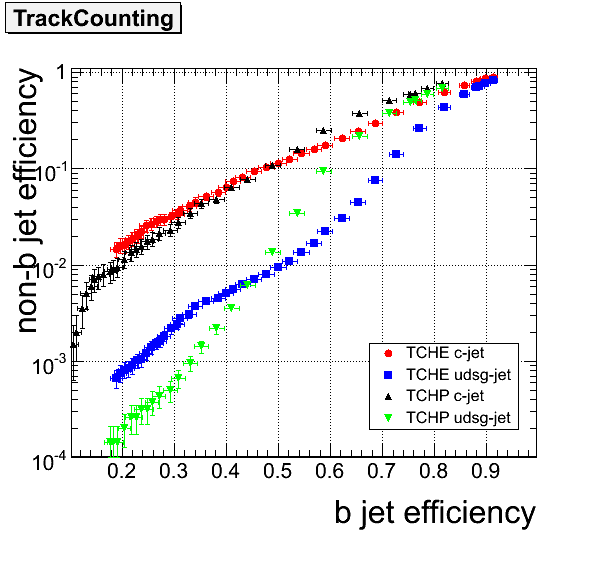
\includegraphics[width=80mm]{Figures/Performance_plot_TC.png}
    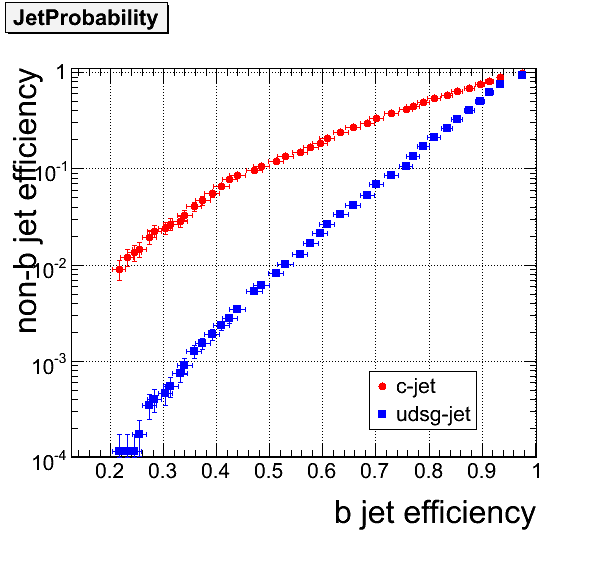
\includegraphics[width=80mm]{Figures/Performance_plot_TP.png}
  \end{center}
  \caption{b-tagging performance measured using the MC truth information 
on the QCD sample with $80<\hat{p_T}<120\;{\rm GeV}/c$ for the TrackCounting 
(top) and the JetProbability tagger(bottom).}
  \label{fig:Performance_plots}
\end{figure}

\begin{table} [th]
\begin{center}
\begin{tabular}{|l|c|l|c|} 
\hline
Algorithm         & Discriminator & Algorithm      & Discriminator\\ \hline
Track Counting    &               & JetProbability &              \\
Loose  (TCL)      &  $TCHE>2.0$   & Loose  (JPL)   &  $>0.26$\\ 
Medium (TCM)      &  $TCHE>4.6$   & Medium (JPM)   &  $>0.50$\\ 
Tight  (TCT)      &  $TCHP>4.7$   & Tight  (JPT)   &  $>0.76$\\ 
\hline
\end{tabular}
\caption{\label{tab:OperatingPoints} 
 Operating points for the TrackCounting and the JetProbability algorithms,
 determined  from MC truth, for jets with $p_T>20$~\gevc and $|\eta|<2.5$.}
 \end{center}
\end{table}

\clearpage

\label{sec:taggingalgos}

\section{Event Observable Distributions}


\subsection{Jet Kinematics}
\begin{figure}[htbp]
  \begin{center}
    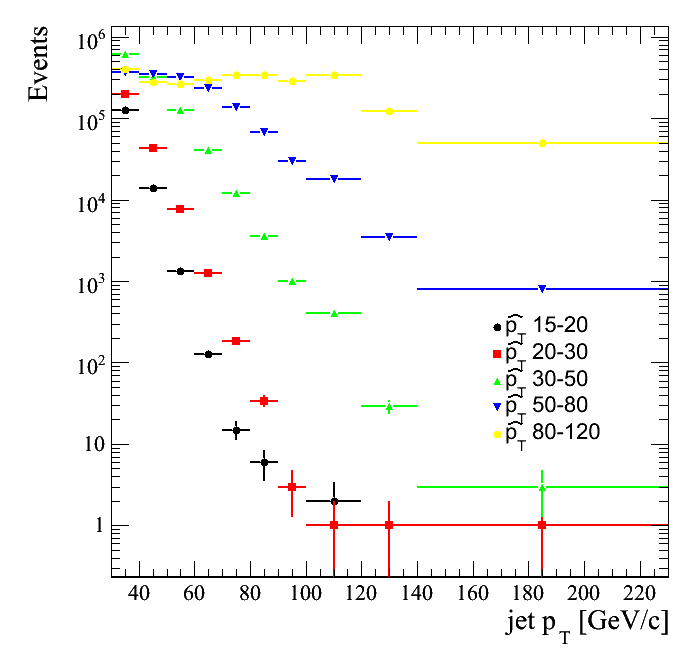
\includegraphics[width=60mm]{Figures/jet_ptqcdbinned.png}
    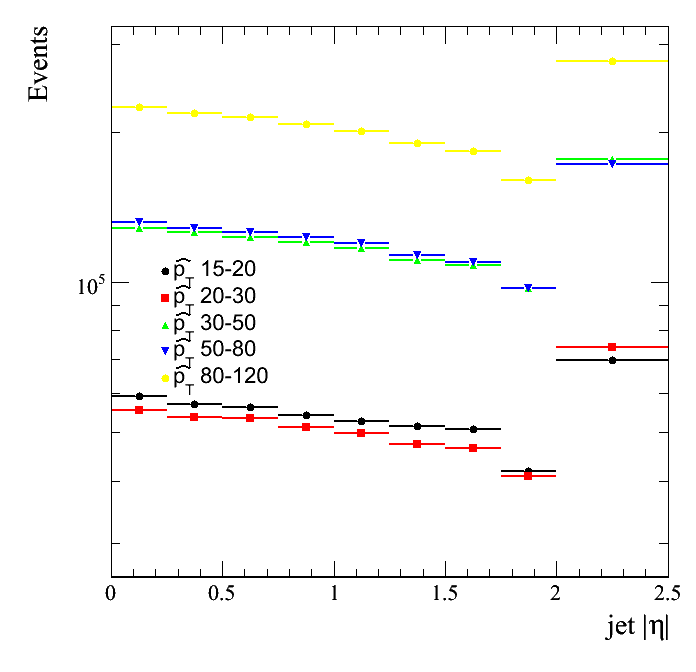
\includegraphics[width=60mm]{Figures/jet_eta_qcdbinned.png}
  \end{center}
  \caption{Jet pT from QCD.}
  \label{fig:jet_pt_QCD}
\end{figure}

\begin{figure}[htbp]
  \begin{center}
    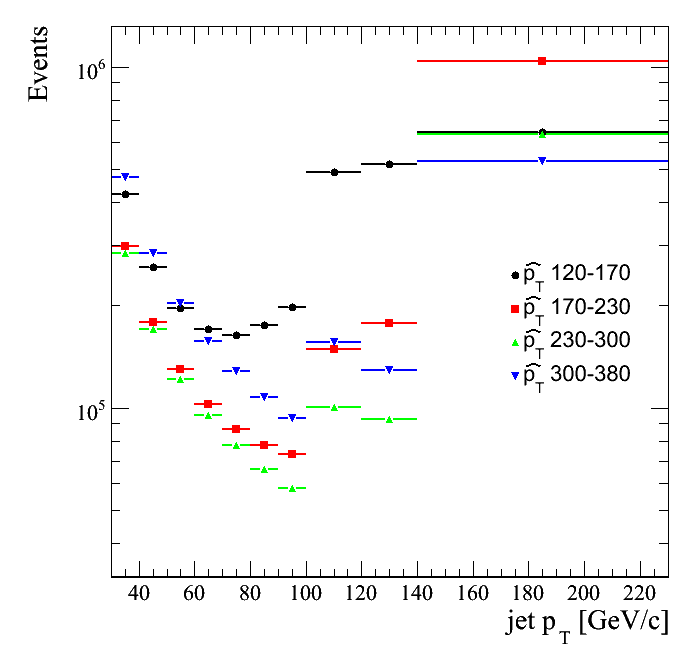
\includegraphics[width=60mm]{Figures/jet_pt2qcdbinned.png}
    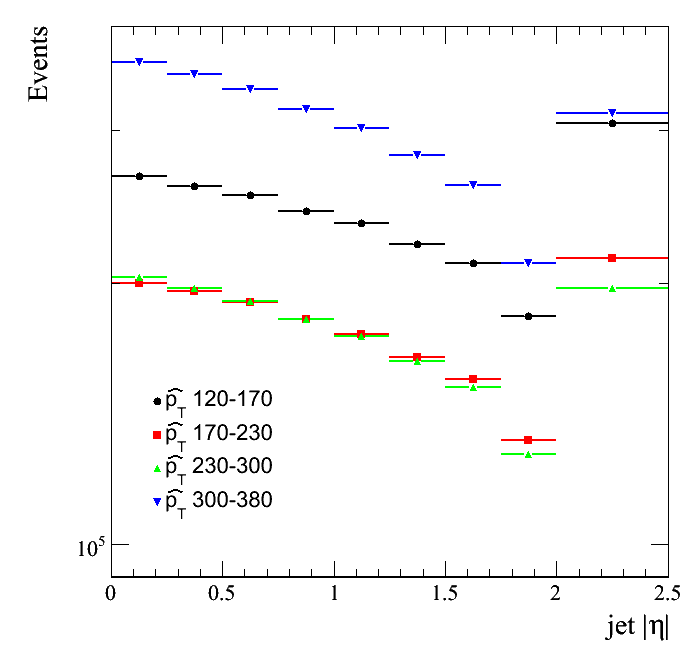
\includegraphics[width=60mm]{Figures/jet_eta_qcdbinned2.png}
  \end{center}
  \caption{Jet pT from QCD.}
  \label{fig:jet_pt_QCD2}
\end{figure}

\begin{figure}[htbp]
  \begin{center}
    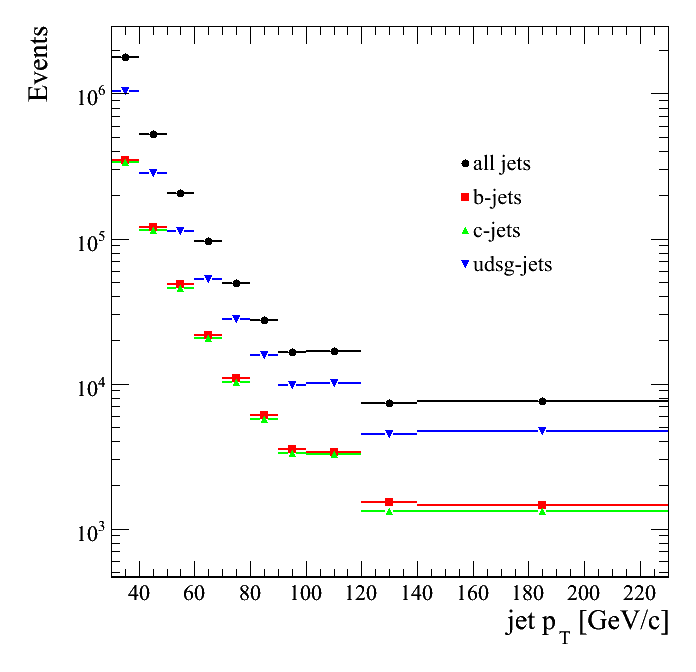
\includegraphics[width=60mm]{Figures/jet_pt_muX.png}
    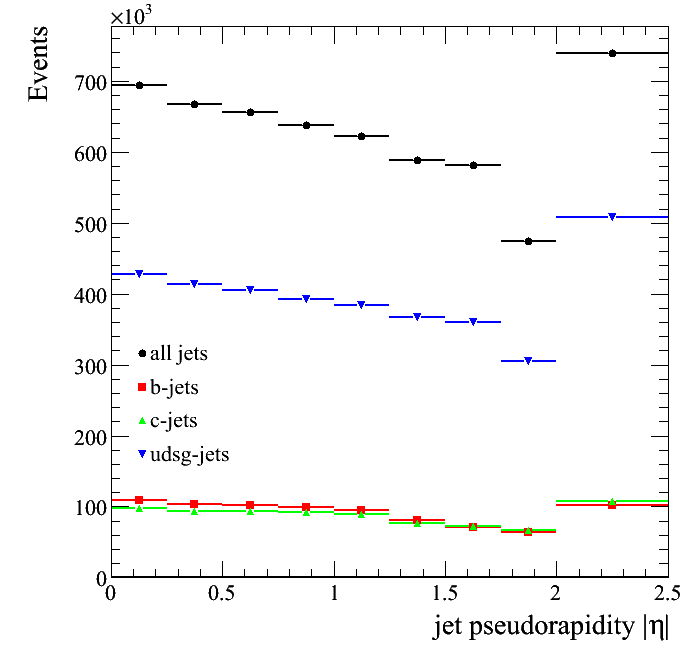
\includegraphics[width=60mm]{Figures/jet_eta_muX.png}
  \end{center}
  \caption{Jet pT and eta from muX.}
  \label{fig:jet_pt_QCD}
\end{figure}

\begin{figure}[htbp]
  \begin{center}
    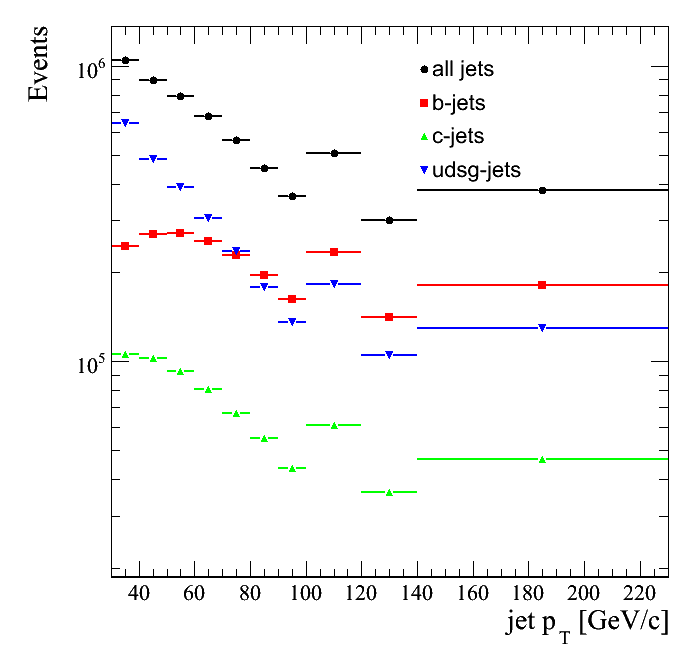
\includegraphics[width=60mm]{Figures/jet_pt_tt0j.png}
    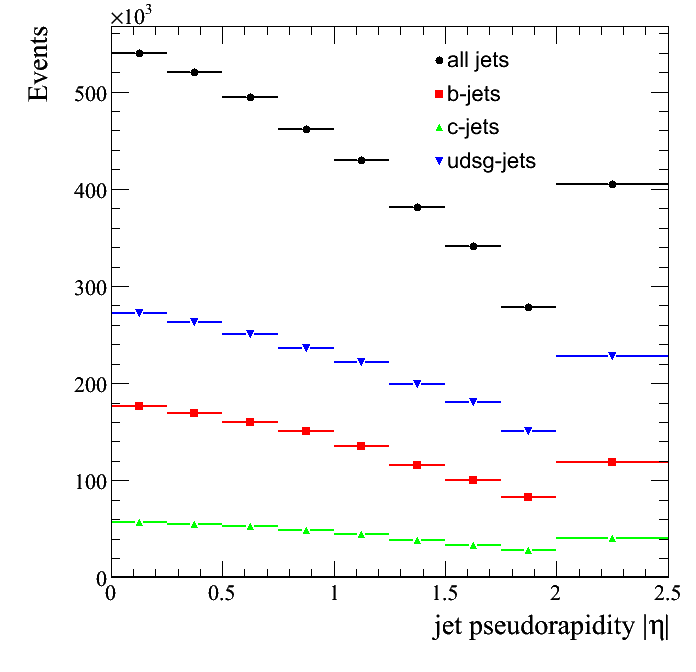
\includegraphics[width=60mm]{Figures/jet_eta_tt0j.png}
  \end{center}
  \caption{Jet pT and eta from ttbar+0jets.}
  \label{fig:jet_pt_QCD}
\end{figure}

\clearpage

\subsection{Muon $p_T$ with respect to muon+jet axis ($p_{Trel}$)}

\begin{figure}[htbp]
  \begin{center}
    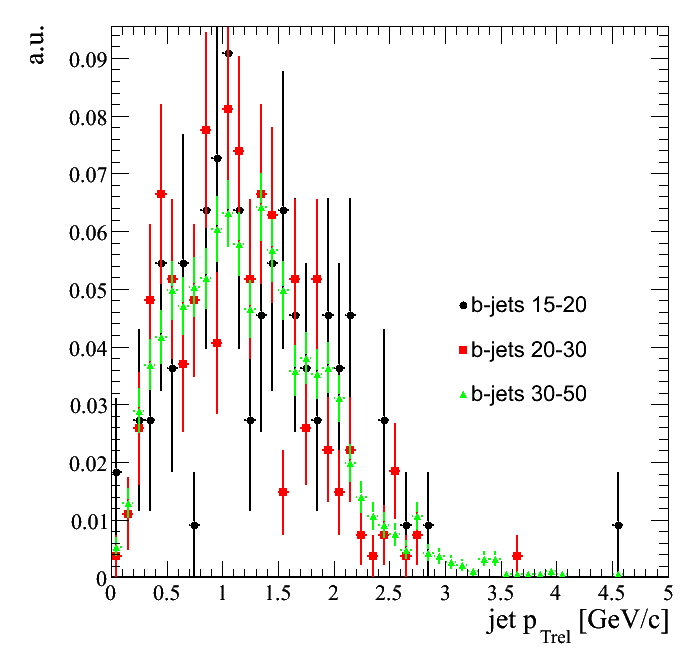
\includegraphics[width=60mm]{Figures/jet_ptrel_qcdbinned.png}
    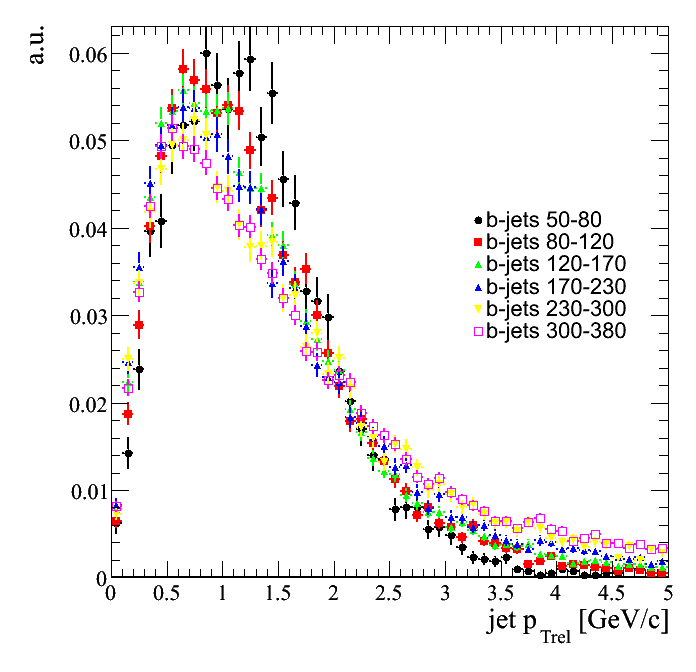
\includegraphics[width=60mm]{Figures/jet_ptrel2qcdbinned.png}
  \end{center}
  \caption{pTrel from b-jets.}
  \label{fig:jet_ptrel}
\end{figure}

\begin{figure}[htbp]
  \begin{center}
    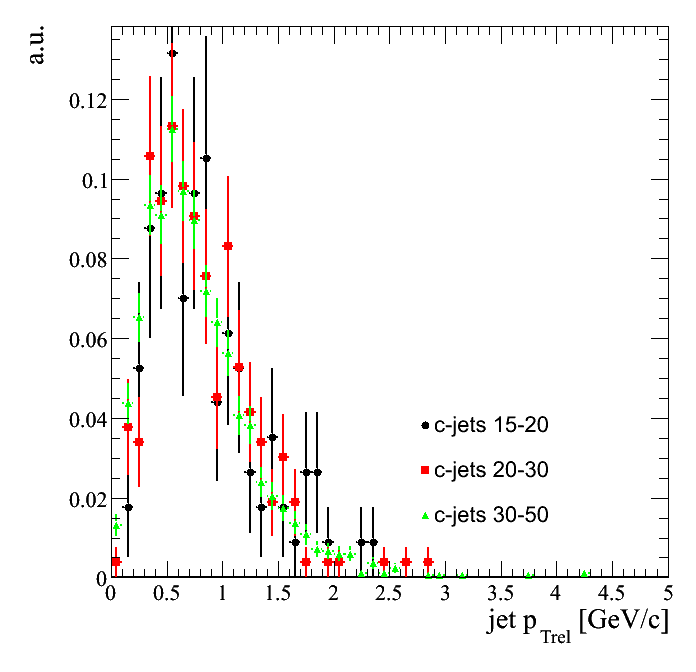
\includegraphics[width=60mm]{Figures/jet_ptrelcqcdbinned.png}
    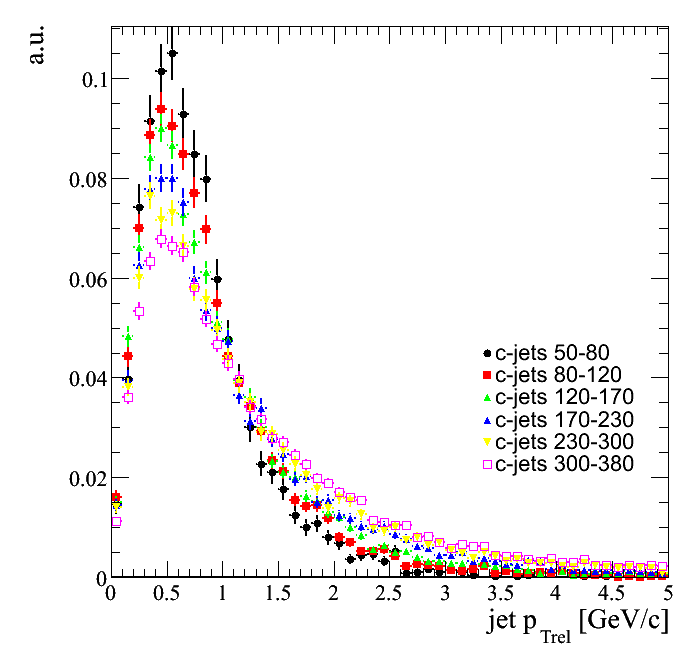
\includegraphics[width=60mm]{Figures/jet_ptrelcqcdbinned2.png}
  \end{center}
  \caption{pTrel from c-jets.}
  \label{fig:jet_ptrel}
\end{figure}


\begin{figure}[htbp]
  \begin{center}
    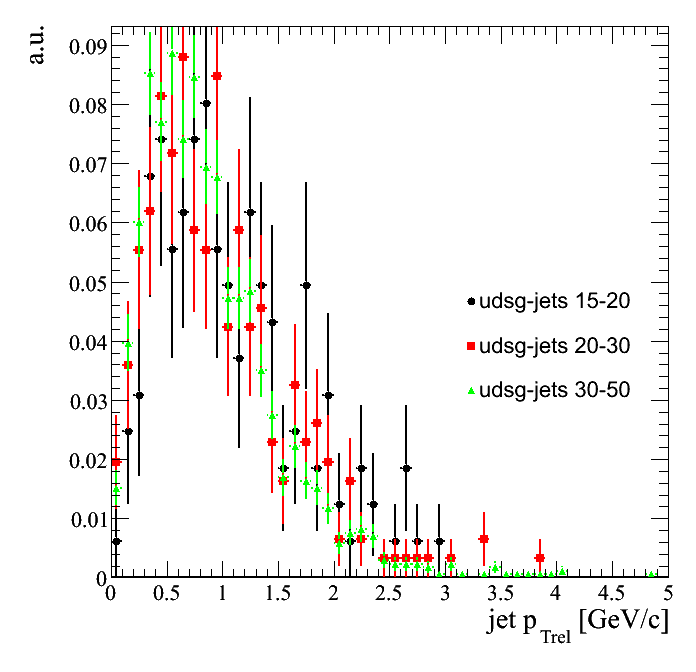
\includegraphics[width=60mm]{Figures/jet_ptreludsgqcdbinned.png}
    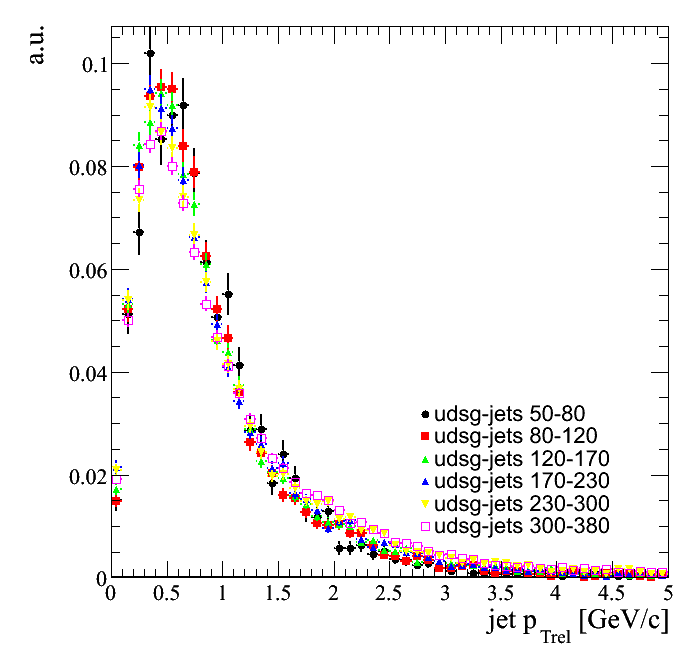
\includegraphics[width=60mm]{Figures/jet_ptreludsgqcdbinned2.png}
  \end{center}
  \caption{pTrel from udsg-jets.}
  \label{fig:jet_ptrel}
\end{figure}

\begin{figure}[htbp]
  \begin{center}
    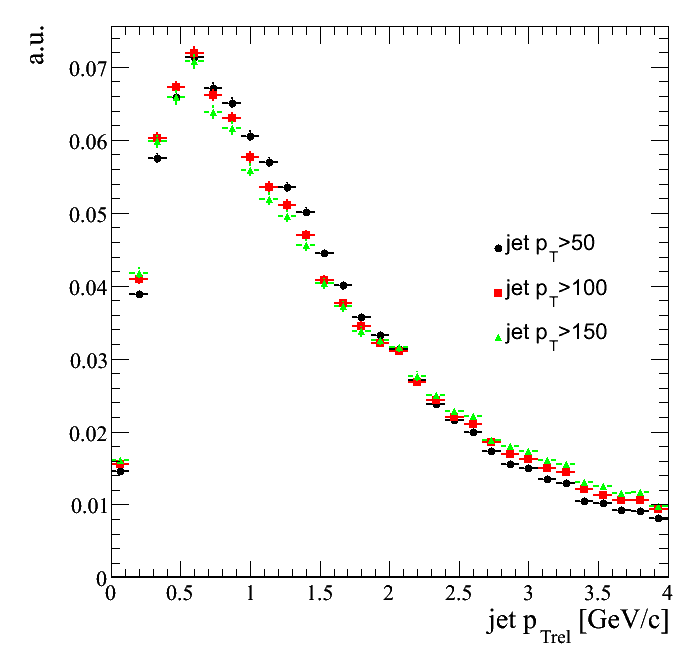
\includegraphics[width=60mm]{Figures/jet_ptrelb_jetcuts.png}
    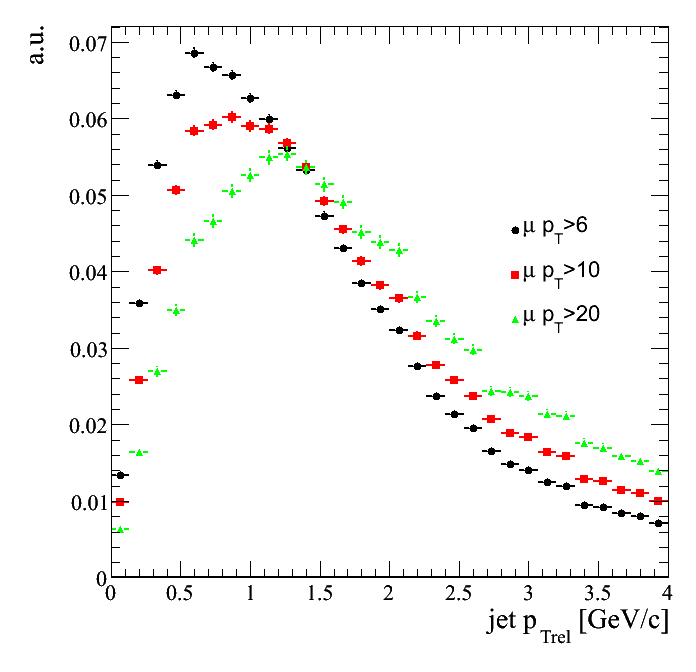
\includegraphics[width=60mm]{Figures/jet_ptrelb_mucuts.png}
  \end{center}
  \caption{pTrel from b-jets for jet and muon cuts.}
  \label{fig:jet_ptrel}
\end{figure}

\begin{figure}[htbp]
  \begin{center}
    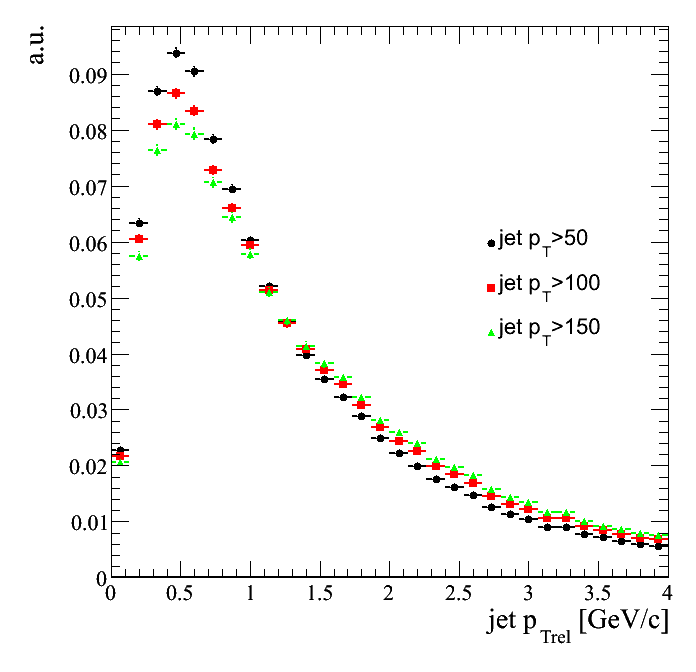
\includegraphics[width=60mm]{Figures/jet_ptrelc_jetcuts.png}
    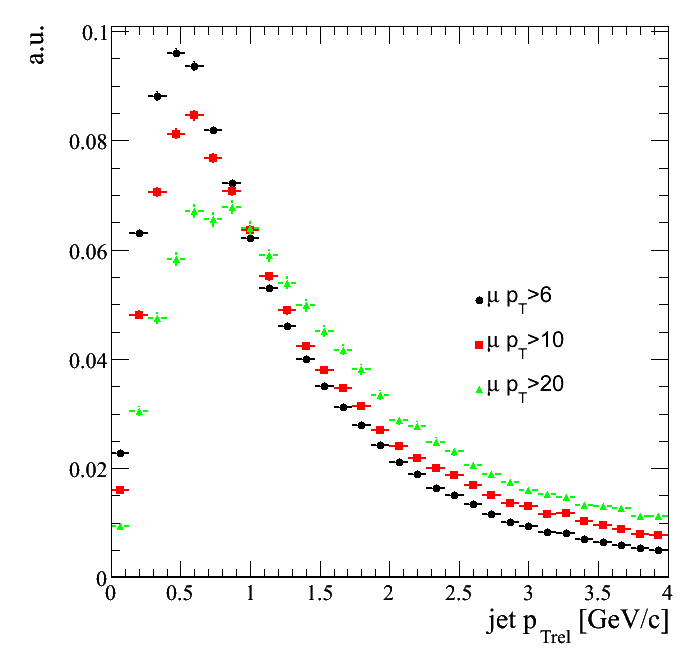
\includegraphics[width=60mm]{Figures/jet_ptrelc_mucuts.png}
  \end{center}
  \caption{pTrel from c-jets for jet and muon cuts.}
  \label{fig:jet_ptrel}
\end{figure}

\begin{figure}[htbp]
  \begin{center}
    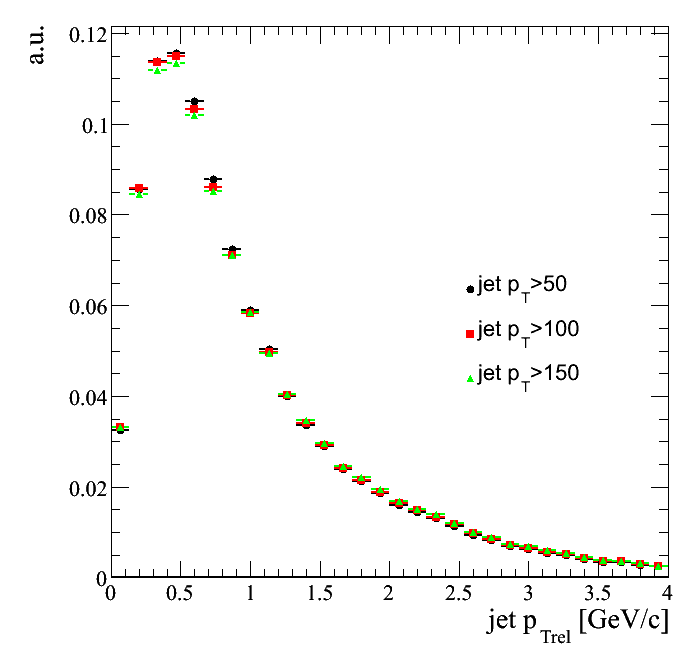
\includegraphics[width=60mm]{Figures/jet_ptreludsg_jetcuts.png}
    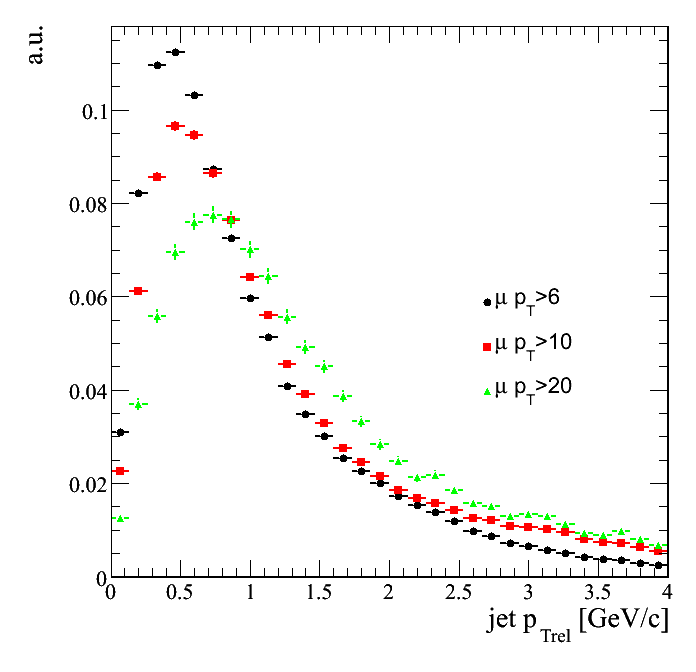
\includegraphics[width=60mm]{Figures/jet_ptreludsg_mucuts.png}
  \end{center}
  \caption{pTrel from udsg-jets for jet and muon cuts.}
  \label{fig:jet_ptrel}
\end{figure}

\begin{figure}[htbp]
  \begin{center}
    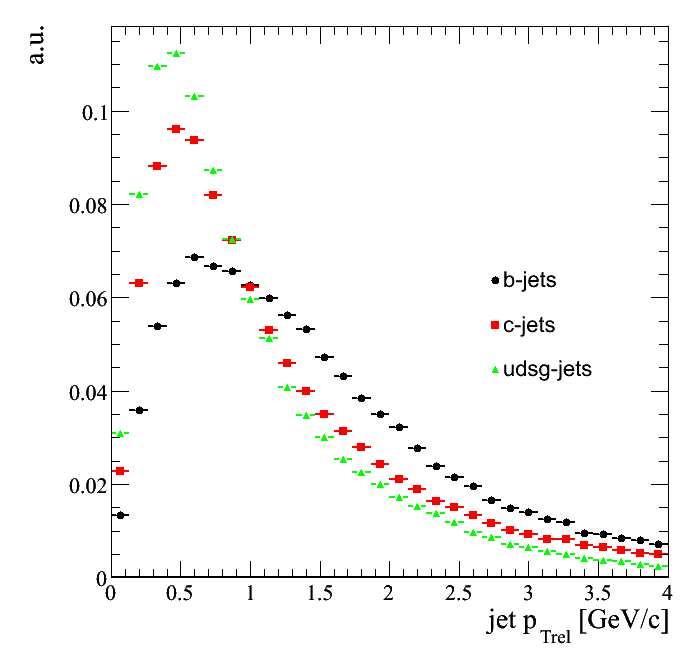
\includegraphics[width=60mm]{Figures/jet_ptrel_mu6.png}
    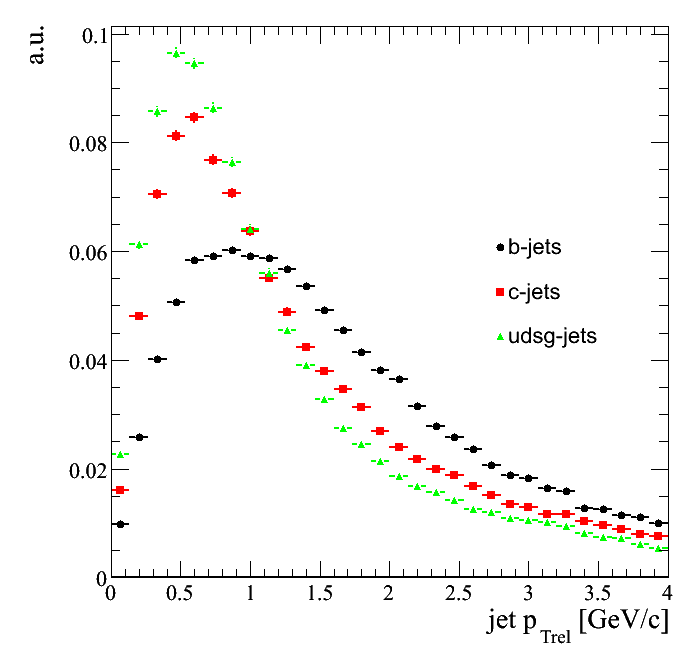
\includegraphics[width=60mm]{Figures/jet_ptrel_mu10.png}
    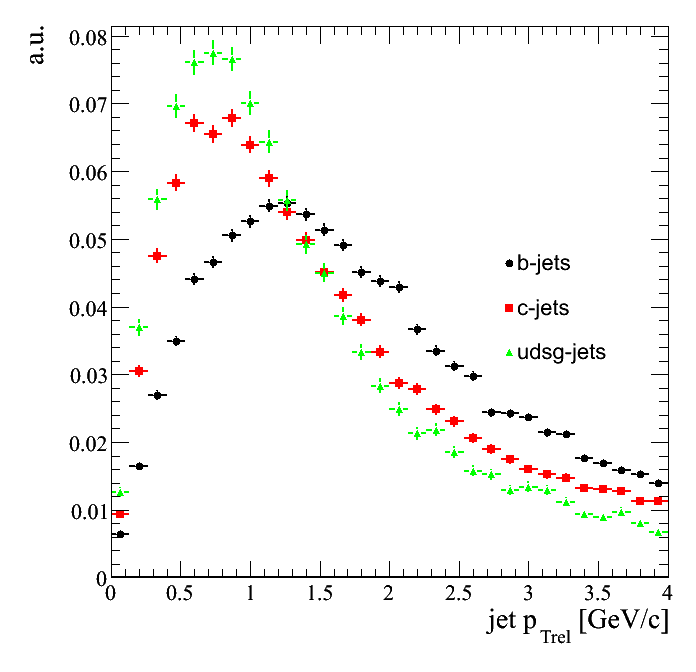
\includegraphics[width=60mm]{Figures/jet_ptrel_mu20.png}
  \end{center}
  \caption{pTrel for muon cuts.}
  \label{fig:jet_ptrel}
\end{figure}

\begin{figure}[htbp]
  \begin{center}
    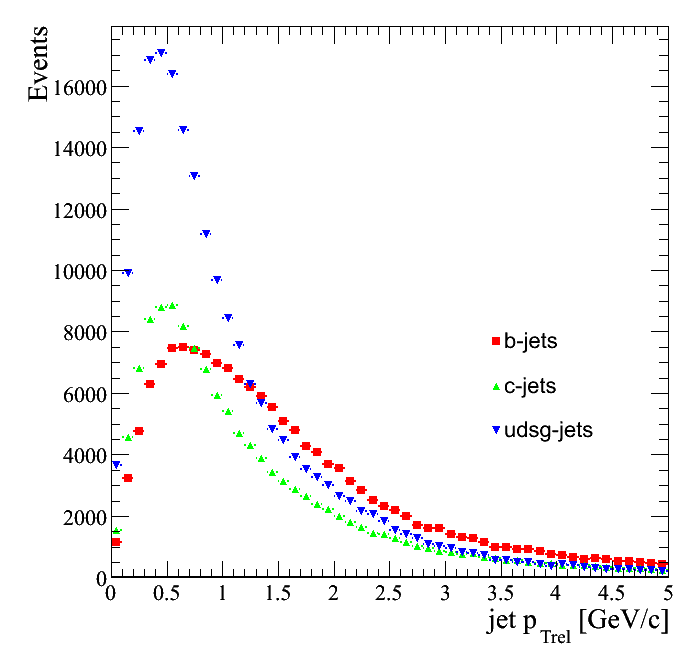
\includegraphics[width=60mm]{Figures/jet_ptrel_allqcd.png}
    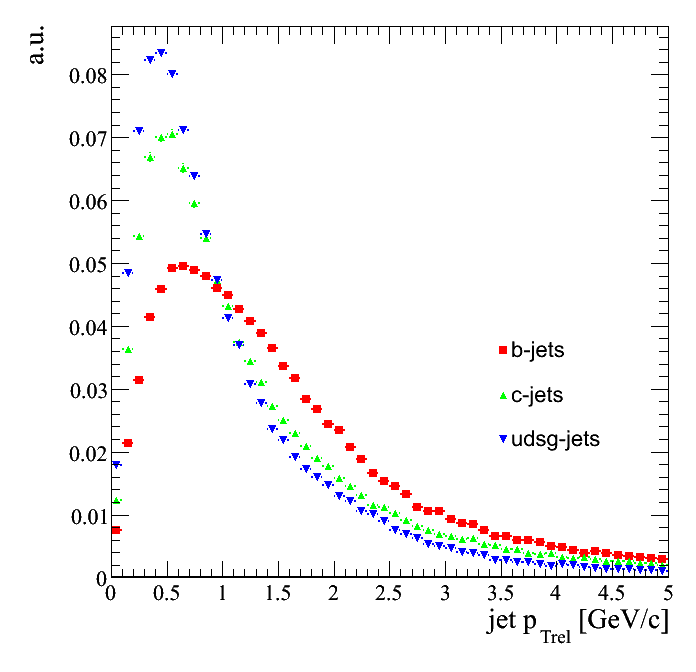
\includegraphics[width=60mm]{Figures/jet_ptrel_norm_allqcd.png}
  \end{center}
  \caption{pTrel from all QCD.}
  \label{fig:jet_ptrel}
\end{figure}


\begin{figure}[htbp]
  \begin{center}
    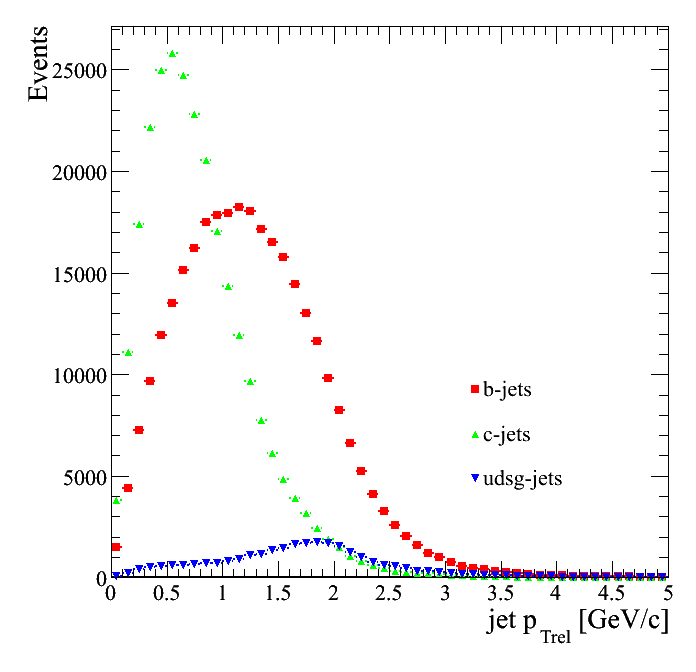
\includegraphics[width=60mm]{Figures/jet_ptrel_muX.png}
    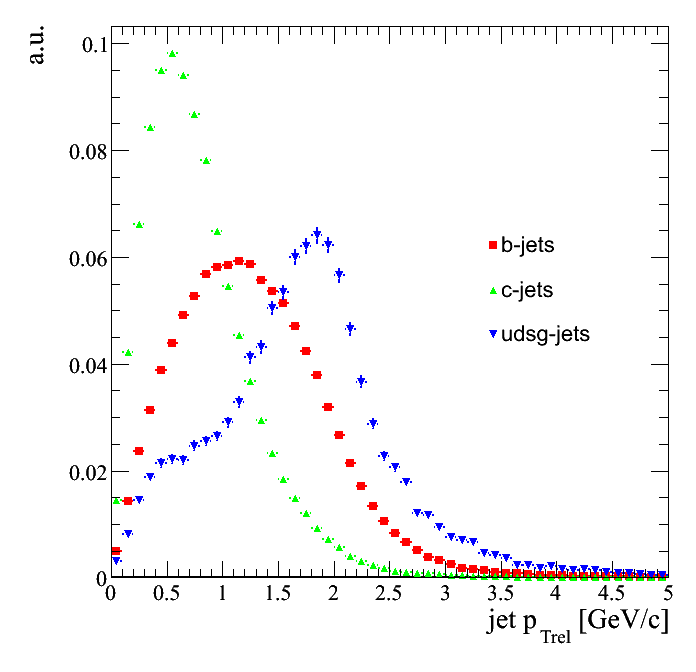
\includegraphics[width=60mm]{Figures/jet_ptrel_norm_muX.png}
  \end{center}
  \caption{pTrel from muX.}
  \label{fig:jet_ptrel}
\end{figure}


\begin{figure}[htbp]
  \begin{center}
    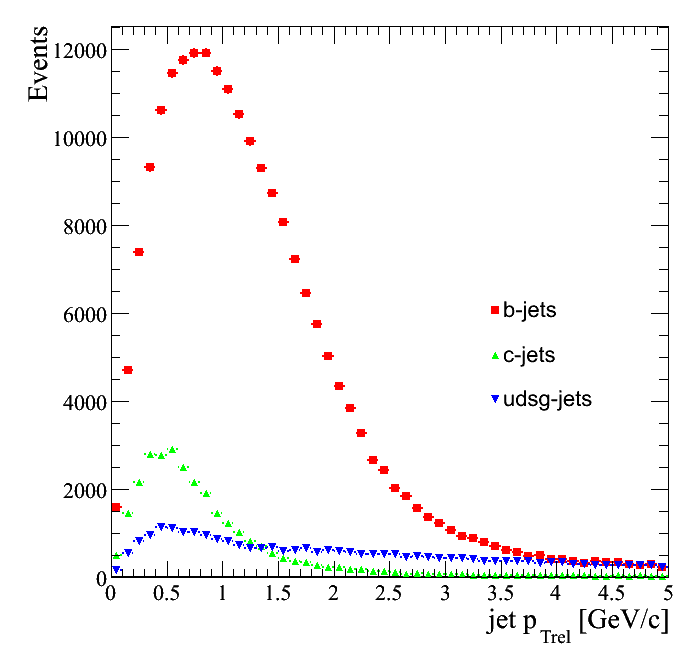
\includegraphics[width=60mm]{Figures/jet_ptrel_tt0j.png}
    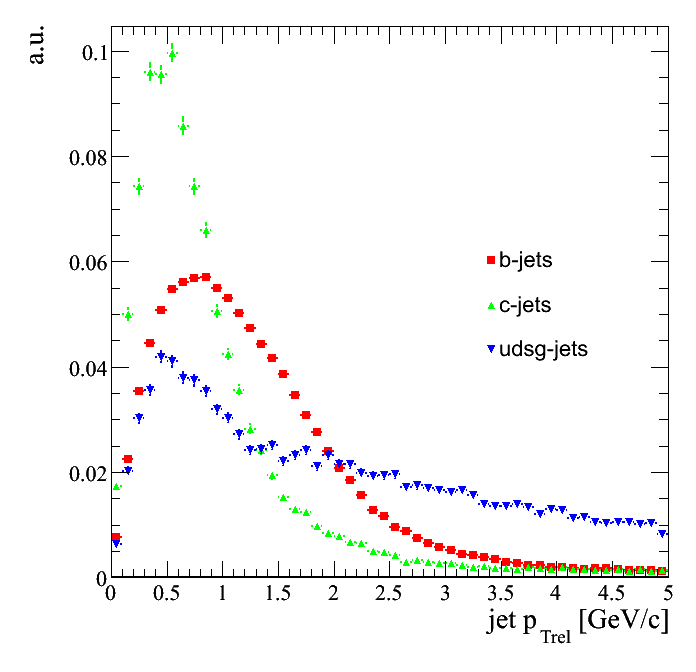
\includegraphics[width=60mm]{Figures/jet_ptrel_norm_tt0j.png}
  \end{center}
  \caption{pTrel from muX.}
  \label{fig:jet_ptrel}
\end{figure}



\label{sec:distributions}

\clearpage
\section{System8 Method}
\label{sec:system8}

The System8 method was initialy studied within CMS in~\cite{ref:btag_oldnote}. Since then it has been 
improved to include the correlation factors for the soft muon tagger:
 $\delta $ and $\gamma$. In the case of multiple real solutions when 
We have also included a criteria to choose the best solution 
When solving the system of equations with a iterative procedure
 
For the current implementation of the System8 method, 
two data samples are used: the muon-in-jet+away-jet sample, and the 
muon-in-jet+tagged-away-jet sample. The lifetime tag (TrackCounting or 
JetProbability) and the Soft Muon Tag requiring muon  \ptrel $ > 0.8 $\gevc 
are applied individually or together, and labelled ``tag'', and ``SLT '',
 respectively. The jets are also divided in two categories: 
$b$ jets, and $c+$light ($cl$) jets. 

The following system of eight equations is then obtained:

\begin{eqnarray}
n &=& n_b + n_{cl} \nonumber\\
p &=& p_b+ p_{cl}\nonumber\\
n^{\rm{tag}} &=&
\varepsilon_b^{\rm{tag}} n_b + \varepsilon_{cl}^{\rm{tag}} n_{cl} \nonumber\\
p^{\rm{tag}} &=&
\beta \; \varepsilon_b^{\rm{tag}} p_b + \alpha \; \varepsilon_{cl}^{\rm{tag}} p_{cl} \nonumber\\
n^{SLT} &=&
\varepsilon_b^{SLT} n_b + \varepsilon_{cl}^{SLT} n_{cl} \nonumber \\
p^{SLT} &=& \delta \; \varepsilon_b^{SLT} p_b + \gamma \; \varepsilon_{cl}^{SLT} p_{cl} \nonumber\\
n^{\rm{tag},SLT} &=&
\kappa_b \; \varepsilon_b^{\rm{tag}} \varepsilon_b^{SLT} n_b +
\kappa_{cl} \; \varepsilon_{cl}^{\rm{tag}} \varepsilon_{cl}^{SLT} n_{cl} \nonumber\\
p^{\rm{tag},SLT} &=&
\kappa_b \; \beta \; \delta \; \varepsilon_b^{\rm{tag}} \varepsilon_b^{SLT} p_b +
\kappa_{cl} \; \alpha \; \gamma \; \varepsilon_{cl}^{\rm{tag}} \varepsilon_{cl}^{SLT} p_{cl} \;.\nonumber
\end{eqnarray}

The terms on the left hand side represent the total number of muon-in-jets
in each sample before tagging ($n$, $p$) and after tagging with
a lifetime tagger ($n^{\rm{tag}}, p^{\rm{tag}}$), the soft muon tagger ($n^{SLT}}, p^{SLT}$), and both ($n^{\rm{tag},SLT},
 p^{\rm{tag},SLT}$). The eight unknowns on the right hand side of the 
equations consist of the number of $b$ and $c+$light jets in the two samples 
($n_b$, $n_{cl}$, $p_b$, $p_{cl}$),  and the tagging efficiencies for
$b$ and $c+$light jets for the lifetime tag and the soft muon tag
($\varepsilon_b^{\rm{tag}}, \varepsilon_b^{SLT}},
\varepsilon_{cl}^{\rm{tag}}, \varepsilon_{cl}^{SLT}}$).
The method assumes that the efficiency for tagging a jet with both the 
lifetime tag and the  soft muon tag (muon \ptrel  cut) can be calculated 
as the product of the individual efficiencies.
Six additional parameters are needed to solve the system of equations:
$\kappa_b$, $\kappa_{cl}$, $\alpha$, $\beta$, $\delta$ and $\gamma$. 
The first two parameters represent
the correlation between the lifetime tag and the muon requirement for $b$ jets 
($\kappa_b$) and $c+$light jets ($\kappa_{cl}$), respectively. 
They are defined as
\begin{eqnarray}
\kappa_b = \frac{\varepsilon_b^{\rm{tag},SLT}}
{\varepsilon_b^{\rm{tag}}\varepsilon_b^{SLT}} \;\; {\rm{and}} \;\;
{\kappa_{cl} =
\frac{\varepsilon_{cl}^{\rm{tag},SLT}}{\varepsilon_{cl}^{\rm{tag}}\varepsilon_{cl}^{SLT}}}\,.
\end{eqnarray}

The parameters $\beta$ and $\alpha$ represent the ratio of the lifetime tagging efficiencies
for $b$ and $c+$light jets, respectively, corresponding
to the two data samples used to solve System8.
They are defined as
\begin{eqnarray}
\beta =\frac{ \varepsilon_b^{\mbox{tag}} \mbox{from muon-in-jet+tagged-away-jet sample} } 
{ \varepsilon_b^{\mbox{tag}} \mbox{from muon-in-jet+away-jet sample} }\, ,
\end{eqnarray}
\begin{eqnarray}
\alpha =\frac{ \varepsilon_{cl}^{\mbox{tag}} \mbox{from muon-in-jet+tagged-away-jet sample} } 
{ \varepsilon_{cl}^{\mbox{tag}} \mbox{from muon-in-jet+away-jet sample} }\, .
\end{eqnarray}
And the parameters $\delta$ and $\gamma$ represent the ratio of the soft muon
tagging efficiencies for $b$ and $c+$light jets, respectively, corresponding
to the two data samples used to solve System8.
They are defined as
\begin{eqnarray}
\delta =\frac{ \varepsilon_b^{SLT} \mbox{from muon-in-jet+tagged-away-jet sample} } 
{ \varepsilon_b^{SLT} \mbox{from muon-in-jet+away-jet sample} }\, ,
\end{eqnarray}
\begin{eqnarray}
\gamma =\frac{ \varepsilon_{cl}^{SLT} \mbox{from muon-in-jet+tagged-away-jet sample} } 
{ \varepsilon_{cl}^{SLT} \mbox{from muon-in-jet+away-jet sample} }\, .
\end{eqnarray}

The correlation factors have been measured for three operating points of the 
TrackCounting and the JetProbability tagger and presented in 
Figures~\ref{fig:correlation_TC}-~\ref{fig:correlation_TP}.


\begin{figure}[htbp]
  \begin{center}
    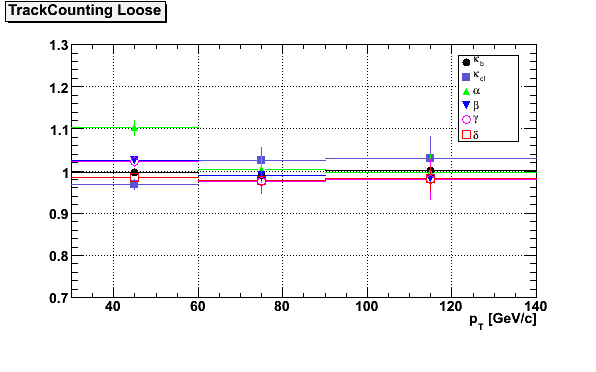
\includegraphics[width=75mm]{Figures/TCL_correlations_ppmux.png}
    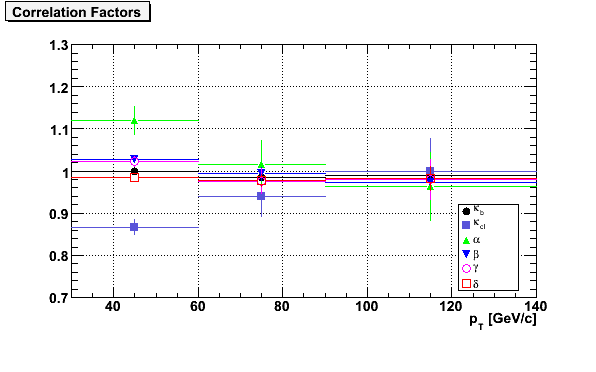
\includegraphics[width=75mm]{Figures/TCM_correlations_ppmux.png}
    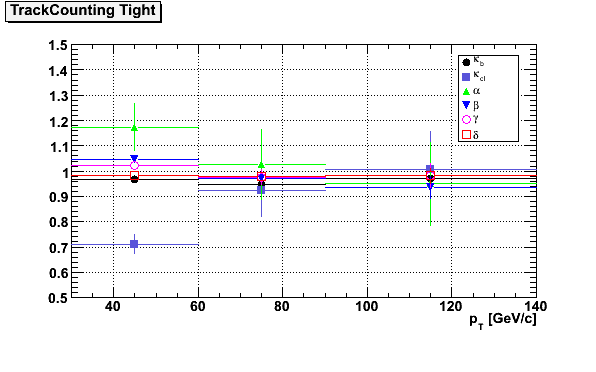
\includegraphics[width=75mm]{Figures/TCT_correlations_ppmux.png}
  \end{center}
  \caption{System8 correlation factors for TrackCounting Tagger as a function
of jet $p_T $ for the loose, medium, and tight operating points.}
  \label{fig:correlation_TC}
\end{figure}

\begin{figure}[htbp]
  \begin{center}
    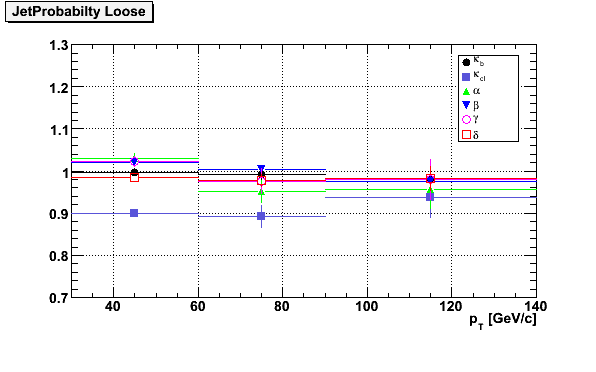
\includegraphics[width=75mm]{Figures/JPL_correlations_ppmux.png}
    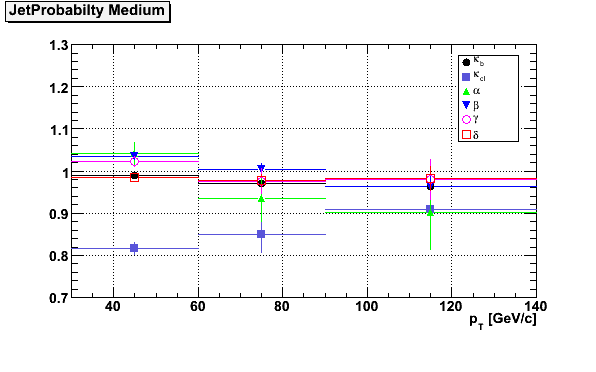
\includegraphics[width=75mm]{Figures/JPM_correlations_ppmux.png}
    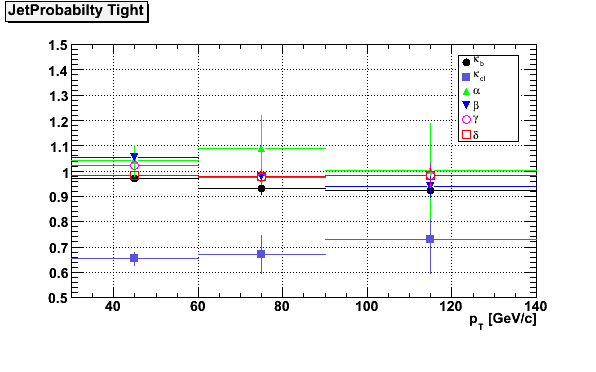
\includegraphics[width=75mm]{Figures/JPT_correlations_ppmux.png}
  \end{center}
  \caption{System8 correlation factors for JetProbability Tagger as a function
of jet $p_T $ for the loose, medium, and tight operating points.}
  \label{fig:correlation_TP}
\end{figure}



\label{sec:system8}
\subsection{System 8 Average Results}
\label{sec:avg_results}

b$-$tag efficiency from System 8 compared to expected efficiency.


\begin{table}[bth]{\small
 \begin{center}
 \begin{tabular}{|l|r@{$\pm$}c|r@{$\pm$}c|r@{$\pm$}c|r@{$\pm$}c|r@{$\pm$}c|r@{$\pm$}c|}
\hline
Sample                 & \multicolumn{4}{|c|}{$pp\rightarrow $\mu$+X$} & \multicolumn{4}{|c|}{$t\bar{t}+0$jets} & \multicolumn{4}{|c|}{QCD} \\ \hline         
Tagger                 & \multicolumn{2}{|c|}{Expected} & \multicolumn{2}{|c|}{System8} & \multicolumn{2}{|c|}{Expected} & \multicolumn{2}{|c|}{System8} & \multicolumn{2}{|c|}{Expected} & \multicolumn{2}{|c|}{System8}  \\ \hline
TCL  & 0.6709 &  0.0014& 0.6610 & 0.0296&  0.7614 & 0.0010& 0.8080 & 0.0637& 0.7853 & 0.0017& 0.7393 & 0.0215\\
TCM  & 0.4983 &  0.0015& 0.5061 & 0.0665&  0.5985 & 0.0012& 0.6527 & 0.0549& 0.6277 & 0.0019& 0.9580 & 0.0815\\
TCT  & 0.2335 &  0.0012& 0.2302 & 0.0133&  0.3191 & 0.0011& 0.3582 & 0.0434& 0.3616 & 0.0019& 0.2936 & 0.0334\\
JPL  & 0.7587 &  0.0013& 0.7653 & 0.0726&  0.8189 & 0.0009& 0.8104 & 0.0200& 0.8056 & 0.0016& 0.6251 & 0.0294\\
JPM  & 0.5257 &  0.0015& 0.5136 & 0.0564&  0.6002 & 0.0012& 0.6083 & 0.0265& 0.5901 & 0.0020& 0.4610 & 0.0687\\
JPT  & 0.2941 &  0.0013& 0.2759 & 0.0080&  0.3630 & 0.0012& 0.3870 & 0.0355& 0.3607 & 0.0019& 0.2665 & 0.0259\\
pTrel& 0.7279 &  0.0013& 0.7324 & 0.0530&  0.6565 & 0.0012& 0.6576 & 0.0096& 0.6863 & 0.0019& 0.6848 & 0.0086\\
 \hline
 \end{tabular}
 \end{center}
\caption[]{Summary of Average System 8 solutions for b$-$tag efficiency.}
\label{tab:b_efficiencies}}
\end{table}




cl$-$tag efficiency from System 8 compared to expected efficiency.


\begin{table}[bth]{\small
 \begin{center}
 \begin{tabular}{|l|r@{$\pm$}c|r@{$\pm$}c|r@{$\pm$}c|r@{$\pm$}c|r@{$\pm$}c|r@{$\pm$}c|}
\hline
Sample                 &\multicolumn{4}{|c|}{$pp\rightarrow $\mu$+X$} &\multicolumn{4}{|c|}{$t\bar{t}+0$jets} & \multicolumn{4}{|c|}{QCD} \\ \hline         
Tagger                 &\multicolumn{2}{|c|}{Expected}&\multicolumn{2}{|c|}{System8}&\multicolumn{2}{|c|}{Expected} & \multicolumn{2}{|c|}{System8}&\multicolumn{2}{|c|}{Expected}&\multicolumn{2}{|c|}{System8}  \\\hline
TCL  & 0.2568& 0.0013& 0.2461& 0.0225& 0.2835& 0.0024& 0.3358& 0.0838& 0.3310& 0.0015& 0.3026& 0.0234 \\
TCM  & 0.0948& 0.0009& 0.1000& 0.0493& 0.1084& 0.0017& 0.1663& 0.0637& 0.1002& 0.0010& 0.0986& 0.0127 \\
TCT  & 0.0158& 0.0004& 0.0133& 0.0143& 0.0203& 0.0008& 0.0713& 0.0459& 0.0224& 0.0005& 0.0074& 0.0041 \\
JPL  & 0.3920& 0.0014& 0.3951& 0.0517& 0.3322& 0.0025& 0.2937& 0.0383& 0.2823& 0.0015& 0.2346& 0.0169 \\
JPM  & 0.1295& 0.0010& 0.1229& 0.0521& 0.1094& 0.0017& 0.1046& 0.0176& 0.0655& 0.0087& 0.0655& 0.0094 \\
JPT  & 0.0277& 0.0005& 0.0171& 0.0041& 0.0260& 0.0008& 0.0420& 0.0084& 0.0210& 0.0005& 0.0018& 0.0031 \\
pTrel& 0.4154& 0.0014& 0.4158& 0.0374& 0.4538& 0.0026& 0.4751& 0.0244& 0.6863& 0.0019& 0.6848& 0.0086 \\
 \hline
 \end{tabular}
 \end{center}
\caption[]{Summary of Average System 8 solutions for cl$-$tag efficiency.}
\label{tab:cl_efficiencies}}
\end{table}

\label{sec:avg_results}
\subsection{System 8 Binned Results}
\begin{figure}[htbp]
  \begin{center}
    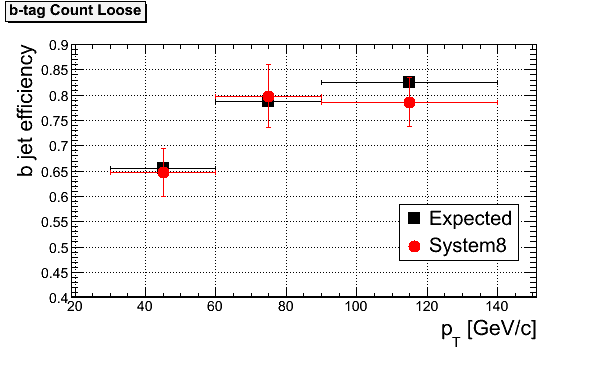
\includegraphics[width=80mm]{Figures/TCL_Tag.png}
    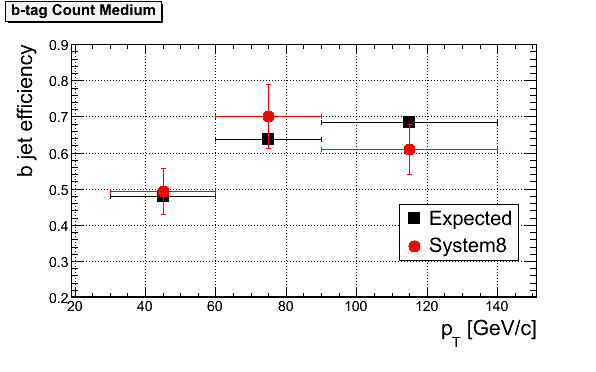
\includegraphics[width=80mm]{Figures/TCM_Tag.png}
    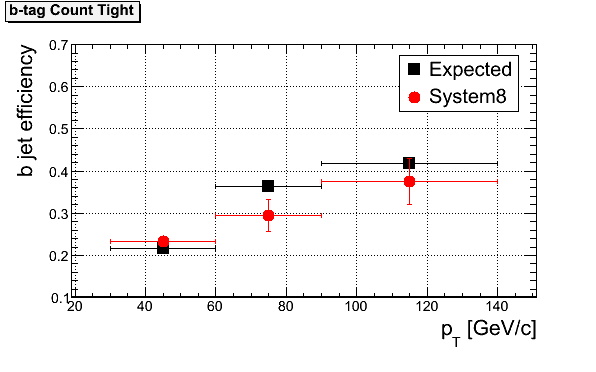
\includegraphics[width=80mm]{Figures/TCT_Tag.png}
    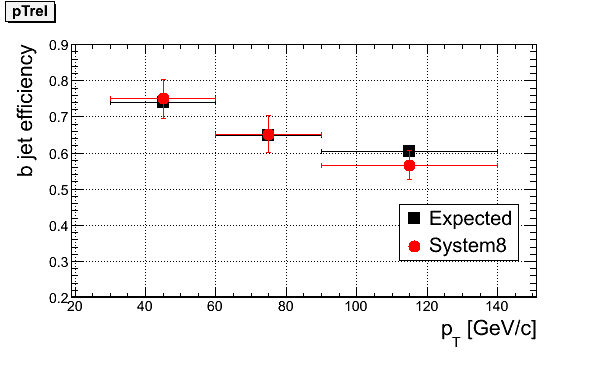
\includegraphics[width=80mm]{Figures/pTrel.png}
  \end{center}
  \caption{Measured and expected b$-$tag efficiency from System8 as a function of jet $p_T $ (requiring $p_T $ $> $ 30 GeV/c).The error bars shown are only statistical errors.}
  \label{fig:S8_TC_results}
\end{figure}


\begin{figure}[htbp]
  \begin{center}
    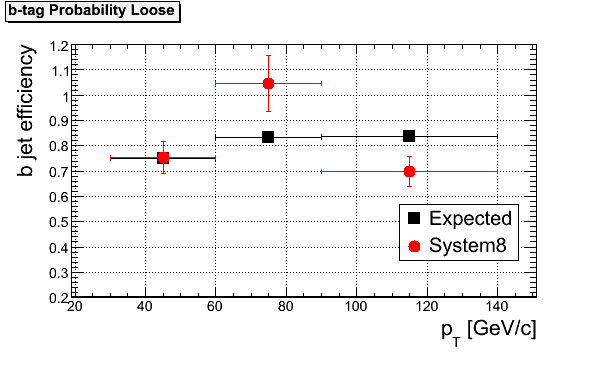
\includegraphics[width=80mm]{Figures/JPL_Tag.png}
    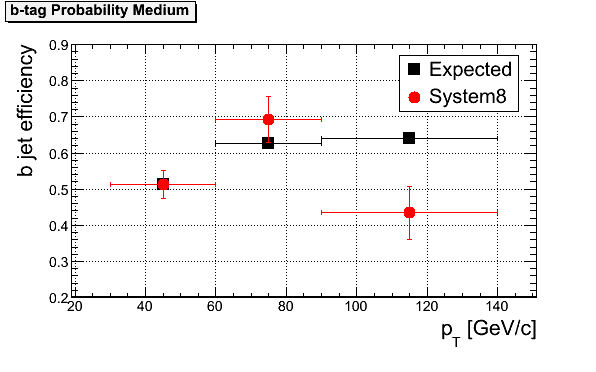
\includegraphics[width=80mm]{Figures/JPM_Tag.png}
    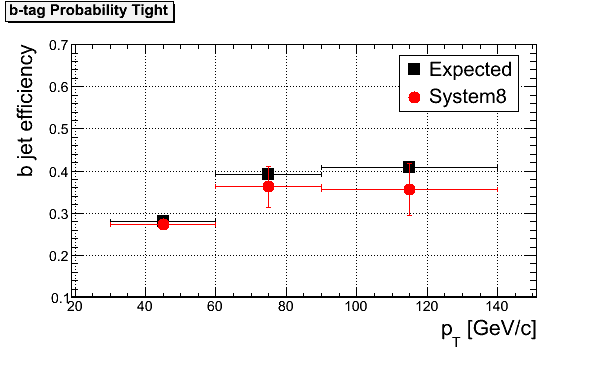
\includegraphics[width=80mm]{Figures/JPT_Tag.png}
  \end{center}
  \caption{Measured and expected b$-$tag efficiency from System8 as a function of jet $p_T $ (requiring $p_T $ $> $ 30 GeV/c).The error bars shown are only statistical errors.}
  \label{fig:S8_JP_results}
\end{figure}

\clearpage


\label{sec:binned_results}

\clearpage
\section{Efficiency of the soft muon tagger}

In this section we use the System8 method to measure the efficiency of a 
simple Soft Muon Tagger (SLT) given by a cut on the \ptrel distribution of the 
muon. To ensure that the two taggers are independent and the correlation 
coefficients are close to unity, we modified the Track Counting tagger.
In the Track Counting tagger for each selected track in a jet, the impact 
parameter significance is computed. The jet is tagged by the Track Counting 
algorithm if the number of tracks with an impact parameter significance 
exceeding a given cut is greater than a discriminator value.

To create a life time tagger not involving the muon track we modified 
the jet track associator. The Jet track associator  loops over all the jets 
in an event and associates the tracks to a jet if they lie within a cone of 
0.5. We modify the Jet track associator to look for the good muons using the
criteria.
\begin{itemize} 
\item   number of Hits in the track $ \ge $ 8;
\item   $\mu $ Pt $ \ge $ 6;
\item   normalized $\chi^{2} \le 5$,
\end{itemize}   
and reject the good muon tracks from the track collection and associate rest 
of the tracks to jets. The modified jets with no muon tracks are then used 
for Track Counting method giving a modified Track counting b-tagging algorithm.

Figure~\ref{fig:Performanceplot} shows the performance plots
 comparing the modified Track Counting tagger with the Track Counting tagger
for the QCD RECO sample in the \pt range 80 to 120 GeV. Even though the 
performance of the Modified Track Counting is somewhat worse, its seperation
power is still sufficient to enrich the sample in b-jets and allow us to use 
System8 to measure the efficiency of the SLT algorithm.


\begin{figure}[htbp]
  \begin{center}
    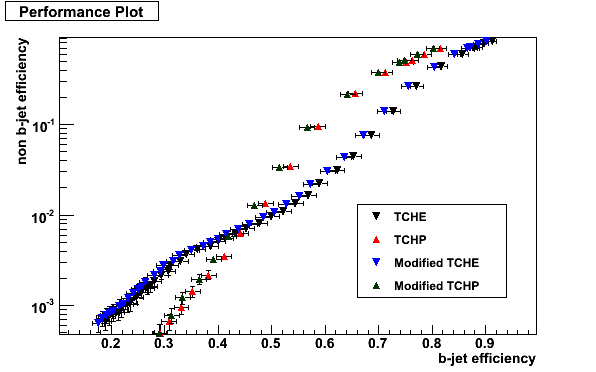
\includegraphics[width=90mm]{Figures/QCD_80_120.png}
  \end{center}
  \caption{Performance Plot comparing the performance of the default and 
modified Track Counting Algorithm for QCD 80-120 GeV sample.}
  \label{fig:Performanceplot}
\end{figure}


The Modified Track Counting tagger has been used as one of the taggers of
System8 to determine the efficiency for the Soft Muon Tagger






\section{Summary and Conclusions}


 The System8 method has been extended to consider correlations for the soft
muon tagger. We now have a better convergence range in jet $p_T$ for System8
method as compared to the previous analysis~\cite{ref:btag_oldnote}. Along with
the b-tagging efficiency we also studdied the charm+light jet tagging 
efficiency using the System8 method. The method was applied to the 
$pp\rightarrow \mu +X$, $t\bar{t}+0$~jets and QCD samples for the three 
operating points of the Track Counting and the Track Probability tagger and the
pTrel(soft muon tagger) . The average solutions from System8 are in good 
agreement with the expected efficiencies obtained from the MC truth information.
The b-tag efficiency has been measured as a function of jet $p_T$ using a coarse
binning in $p_T$ for the $pp\rightarrow \mu +X$ sample. The agreement between 
the measured and expected b-tag efficiency from MC truth is good for the Track 
Counting and pTrel taggers, but the agreement is not very good for the 
Jet Probability tagger for the loose and medium operating points.

 We would like to incorporate some improvements/revisions into the Performance 
measurement package like cross-checking that we use the muon with the highest 
$p_T$ to calculate the pTrel, improving the muon identification, 
using a muon trigger, and try to get rid of the tiny contamination from other 
processes with a muon-in-jet like the $J/\Psi $ and charm quark decay.

\label{sec:conclusions}

\section{Acknowledgment} 
We would like to thank ...

\appendix
%DB \input{Correlations}
%DB \label{sec:correlations}

\begin{thebibliography}{99}

\bibitem{ref:btag_oldnote}
M.~Narain, P.~Tan, F.~Yumiceva, J~.Andrea, D.~Bloch, D.~Gel\'e, P.~Juillot
V.~Bazterra, C.~Gerber, ``Performance Measurement of $b$ tagging Algorithms Using Data containing Muons within Jets'', CMS AN-2007/046 (2007).

\bibitem{ref:csa07}
https://twiki.cern.ch/twiki/bin/view/Main/AlpgenSummer07.

\bibitem{ref:pythia}
T.~Sj{\"o}strand, L.~Lonnblad and S.~Mrenna, hep-ph/0108264 (2001).

\bibitem{ref:alpgen}
M.~L.~Mangano, M.~Moretti, F.~Piccinini, R.~Pittau, and A.~D.~Polosa, ``ALPGEN, a generator for hard multiparton processes in hadronic collisions''. JHEP 07 (2003) 001, arXiv:hep-ph/0206293.

\bibitem{ref:iterativecone5}
P.~Schieferdecker et al., ``Performance of Jet Algorithms in CMS''. CMS Analysis Note 2008/001 (2008).
 
\bibitem{ref:root}
ROOT analysis system 
http://root.cern.ch/

\end{thebibliography}
 
 
%%%%%%%%%%%%%%%%%%%%%%%%%%%%%%%%%%%%%%%%%%%%%%%%%%%%%%%%%%%%%%%%%%%%%%%%%%%%%%%

%%%%%%%%%%%%%%%%%%%%%%%%%%%%%%%%%%%%%%%%%%%%%%%%%%%%%%%%%%%%%%%%%%%%%%%%%%%%%%%
\end{document}
